\section{Stability and Control}

\nomenclature{$d_p$}{Thrust Level}%
\nomenclature{$d_e$}{Elevator setting}%
\nomenclature{$n_z$}{Load factor}%

\subsection{Equilibrium flight}
For the following analysis the following set of kinematic and dynamical
equations describes the motion of the aircraft sufficiently:
\begin{align}
    X - mgsin\theta &= m\big(\dot{u}^E + qw^E - rv^E \big)
    \label{full_longitudinal1}\\
    Y + mgcos\theta sin\phi &= m\bigl(\dot{v}^E+ ru^E - pw^E\bigr)\\
    Z + mgcos\theta cos\phi &= m\big(\dot{w}^E+ pv^E - qu^E\bigr)
    \label{full_longitudinal3}\\
    L &= I_x\dot{p} - I_{zx}\dot{r} + qr\bigl(I_z - I_y\bigr) - I_{zx}pq + qh_z' -
    rh_y'\\
    M &= I_y\dot{q} + rp\bigl(I_x - I_z\bigr)- I_{zx}\bigl(p^2-r^2\bigr) + rh_x' -
    ph_z'\\
    N &= I_z\dot{r} - I_{zx}\dot{p} + pq\bigl(I_y - I_x\bigr) + I_{zx}qr + ph_y'-qh_x'\\
    p &= \dot{\phi} - \dot{\psi}sin\theta\\
    q &= \dot{\theta}cos\phi + \dot{\psi}cos\theta sin\phi\\
    r &= \dot{\psi}cos\theta cos\phi- \dot{\theta} sin\phi \\
    \dot{\phi} &= p + \bigl(qsin\phi+ rcos\phi\bigr)tan\theta\\
    \dot{\theta} &= qcos\phi - rsin\phi\\
    \dot{\psi} &= \bigl(qsin\phi + rcos\phi\bigr)sec\theta\\
    \dot{x_E} &= u^Ecos\theta cos\psi + u^E\big(\sin\phi sin\theta cos\psi -
    cos\phi sin\psi\big) + \notag\\
     &+ w^E\big(\cos\phi sin\theta cos\psi - sin\phi sin\psi\big) \\
    \dot{y_E} &= v^Ecos\theta sin\psi + v^E\big(\sin\phi sin\theta sin\psi +
    cos\phi cos\psi\big) + \notag\\
     &+ w^E\big(\cos\phi sin\theta sin\psi - sin\phi cos\psi\big) \\
    \dot{z_E} &= -u^Esin\theta + v^Esin\phi cos\theta + w^Ecos\phi cos\theta
    \label{full_longitudinal15}\\
    u^E &= u + W_x\\
    v^E &= v + W_y\\
    w^E &= w + W_z \label{full_longitudinal18}
\end{align}

The above equations contain the following assumptions:
\begin{itemize}
\item The airplane is a rigid body, which may have attached to it any number of
rigid spinning rotors.
\item Cxz is a plane of mirror symmetry.
\item The axes of any spinning rotors are fixed in direction relative to the body
axes, and the rotors have constant angular speed relative to the body axes.
\end{itemize}

\subsubsection{Level Flight Trim Conditions}
As in the 1st part of the report, we have to first find a flyable situation for
the aircraft model. This is done by setting as many states of the above
equations to zero.
Equations~\ref{full_longitudinal1},\ref{full_longitudinal3},\ref{full_longitudinal15}
give 3 nonlinear algebraic equations. We also choose to set $\dot{M} = 0$ and
also know the formula for the velocity magnitude, $V = u^2 + v^2$ since $w = 0$.

So we end up with the following set of equations which we solve to compute the
trimmed state.

\begin{align}
    X - mgsin\theta &= 0\\
    Z + mgcos\theta &= 0\\
    -u^Esin\theta +  w^Ecos\theta &= 0\\
    \dot{M} &= 0\\
    V^2 &= u^2 + v^2
\end{align}
\begin{center}Set of nonlinear equations for trimmed state\end{center}

After finding an initial flyable situation, we linearise initial set of 
differential equations so that we end up with a system of the form:
\begin{align*}
    \underline{\dot{x}} &= \rttensor{J}\underline{\Delta x} +
    \rttensor{B}\underline{\Delta c}\\
    \underline{y} &= \rttensor{C}\underline{\Delta x}
\end{align*}
where for negligible input the differential equations are trimmed down to the 
$\underline{\dot{x}} = \rttensor{J}\,\underline{\Delta x}$ linear system.

Executing this procedure for mach numbers in the range of 0.1-0.7 and altitudes
0, 5000, 10000m we obtain the following graphs for $alpha, \delta_e,\delta_p$:

\begin{figure}[H]
    \centering
    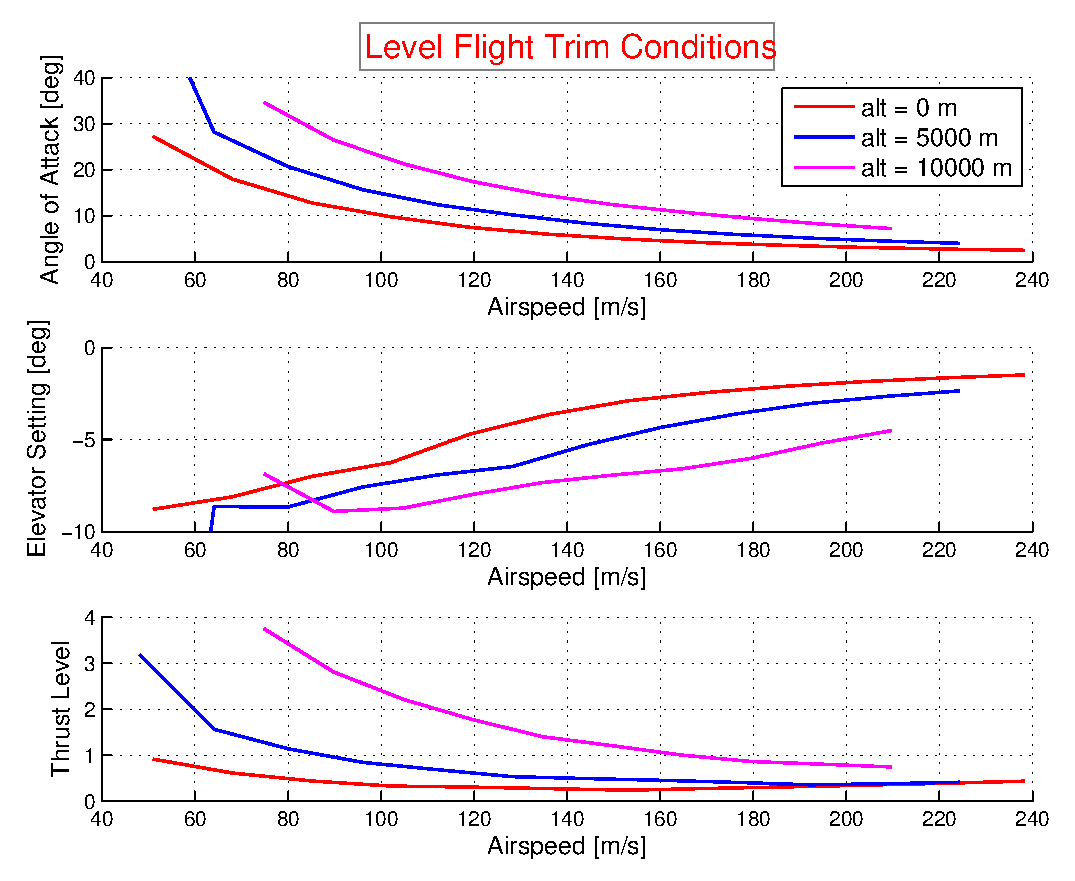
\includegraphics[width=1.0\textwidth]{equilibrium_conditions}
    \caption{$alpha, \delta_e,\delta_p$ for the trimmed Model}
\label{fig:equilibrium_conditions}
\end{figure}


\subsubsection{Center of gravity influence}
To investigate the influence of the center of gravity (xcg) on the elevator
angle we plot the equilibrium elevator as a function of the airspeed for
an altitude of 5000m  for two different xcg values (10.0, 10.3)m. 
The result is shown in fig~\ref{fig:xcg_investigation}.

\begin{figure}[H]
    \centering
    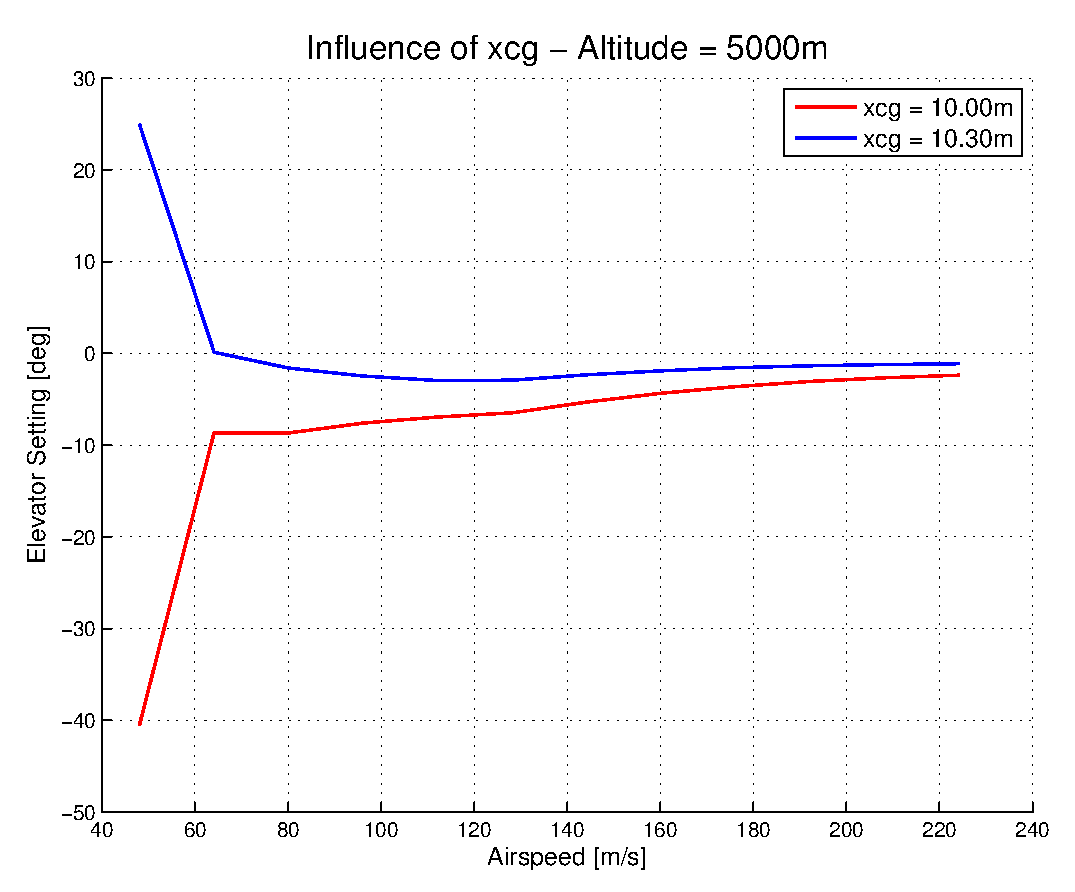
\includegraphics[width=1.0\textwidth]{xcg_investigation}
    \caption{Elevator setting for different cg positions}
    \label{fig:xcg_investigation}
\end{figure}

As we can see the sign of the setting changes to positive
\footnote{The elevator setting is defined as positive when the elevator goes
down.} at low airspeed. This is because the center of gravity has moved further
away from the tip of the aircraft comparing to the aerodynamic center, so a
torque emerges pushing the nose of the aircraft upwards. So in order for the
pitch-motion to be stable the elevator has to be positive as it is when xcg =
10.3m. So we can conclude that since the elevator setting is positive for a wide
range of airspeeds, xcg = 10.3m is not allowed position for the
aircraft. 

\subsubsection{Elevator per g}
The \textit{Elevator per g} can be computed using the following formula:
\begin{equation}
    Elevator_per_g = \frac{\Delta \delta e}{n-1}
    \label{eqn:elevator_per_g}
\end{equation}

In order to find it, we hold the velocity constant and the the thrust level zero,
for certain altitude and we implement a step input to the elevator. We then take
measure the difference in the load factor and therefore compute the elevator per
g from eq.~\ref{eqn:elevator_per_g}. 
We end up with the followign results which show that the epg goes down as the altitude increases.
\footnote{The results are also handed in as logfiles, see elevetor\_per\_g.log}:
\begin{itemize}
    \item $Altitude = 0 m\rightarrow Epg = 16.660$
    \item $Altitude = 5000 m \rightarrow Epg = 5.892$
    \item $Altitude = 10000 m \rightarrow Epg = 1.792$
\end{itemize}


\subsection{Linear stability analysis}

In order to investigate the linear stability of the aircraft we have to perform
an eigenvalue analysis for the Jacobian matrix computed during the trim problem
% todo add ref to previous equation

We compute the eigenvalues for altitudes 0, 5000, 10000m and for mach numbers
in the range of 0.1 - 0.7. We then plot the root locus graphs of the
eigenvalues with airspeed as a parameter.

\begin{figure}[H]
    \centering
    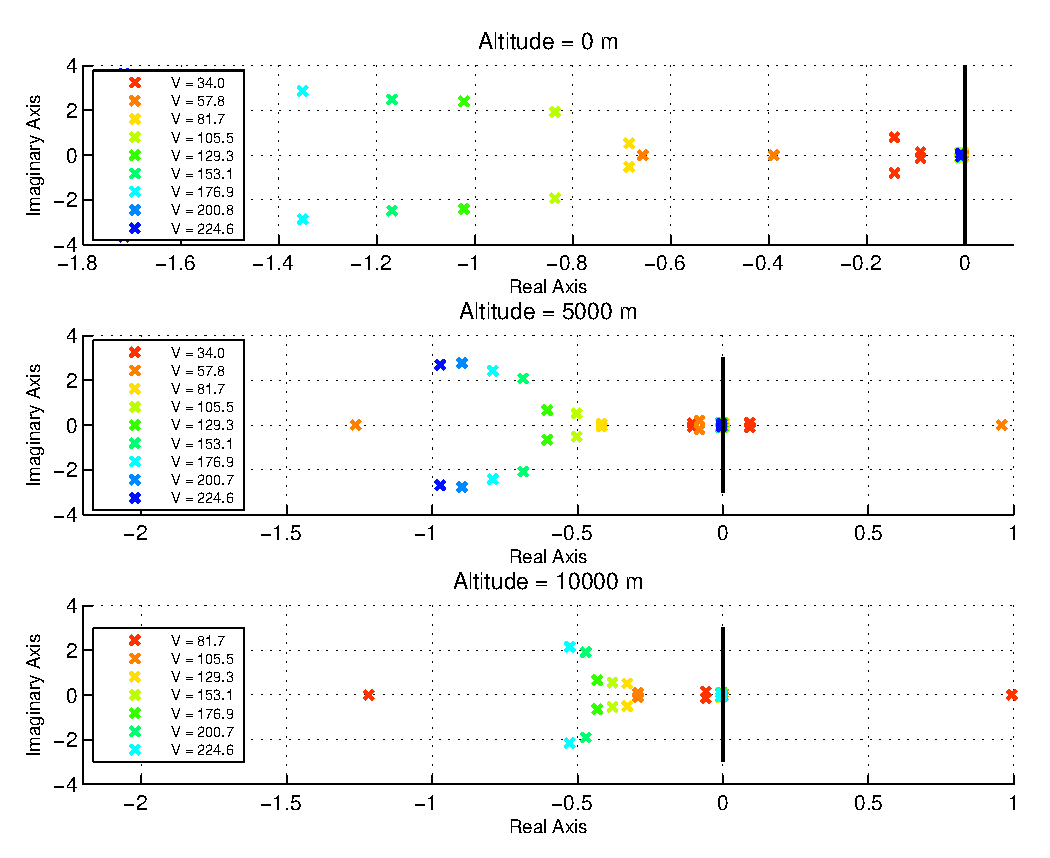
\includegraphics[width=1.0\textwidth]{linear_stability}
    \caption{Root Locus graph with regards to the airspeed}
    \label{fig:rlocus_airspeed}
\end{figure}

From fig.~\ref{fig:rlocus_airspeed} we can see that the linearised model
\textit{is not stable} for low airspeeds at alitude increases. More
specifically, at h = 5000m, the system is unstable for $V = 34\sfrac{m}{s}$
and $V = 57.8\sfrac{m}{s}$ and it becomes stable as the airspeed increases to 
$81.7\sfrac{m}{s}$. For h = 10000m on the other hand, we could not even reach an 
equilibrium trim state for $V \leq 81.7 {m}{s}$.

In particular, because we are interested in the stability of the longitudinal
movement we investigate the behavior of a submatrix of J that corresponds to the
longitudinal equations \cite{etkin_dynamics_1972}.

\begin{equation}
    J' = J\big(\Delta \dot{u}, \dot{w}, \dot{q}, \Delta
    \dot{theta}\big)\label{eqn:Jlong}
\end{equation}

For the stability analysis we compute the following based on J':
\begin{itemize*}
    \item Eigenvalues $\lambda$
    \item Eigenvectors $v$
    \item Oscillation frequencies $f$
    \item Time to half/double
\end{itemize*}

To compute the eigenvalues and eigenvectors, we implement the following
methodology:
\begin{align*}
    J' v &= \lambda v \Rightarrow\\
    \big(J'-\lambda I\big)v &= 0 \Rightarrow\\
    \abs{J' - \lambda I} &= 0 \numberthis \label{eqn:eigs_calc}
\end{align*}

Using eq~\eqref{eqn:eigs_calc} we can calculate the eigenvalues of the matrix by
solving the polynomial equation. Then to compute the corresponding eigenvector
we substitue each $\lambda$ calculated in the inital equation:
\begin{equation}
    \big(J'-\lambda_i I\big)v_i = 0,\; for\,i=1,\dots N,
    \label{eqn:eigvs_calc}
\end{equation}
where N is the total number of eigenvalues 

We also know that since the eigenvalues computed are of the form $n \pm
i\omega$, the frequency of each oscillation mode can be computed directly from
the eigenvalues:
\begin{equation}
    f = \frac{\omega}{2 \pi}
\end{equation}

The time to double/half can also be obtained using the following formula 
\cite{etkin_dynamics_1972}.

\begin{equation}
    t_{double} = t_{half} = \frac{log_e2}{\abs{n}}
    \label{eqn:time2double}
\end{equation}

Finally having computed the eigenvalues and the corresponding eigenvectors, the
oscillation modes can be computed using the following expression:
\begin{equation}
    \mathbf{X} = \mathbf{X_0}e^{\lambda t}
\end{equation}

The results of the eigenvalue analysis are presented in the appendix of the report
and are also handed in as logfiles.

\subsection{Nonlinear simulation}
We now simulate the behavior of the aircraft when executing each one of the
following maneuvers
\begin{itemize*}
    \item Looping
    \item Cobra maneuver
\end{itemize*}

We first run the simulation for 300 seconds with fixed inputs for the elevator
and the thrust level.
\begin{figure}[H]
    \centering
    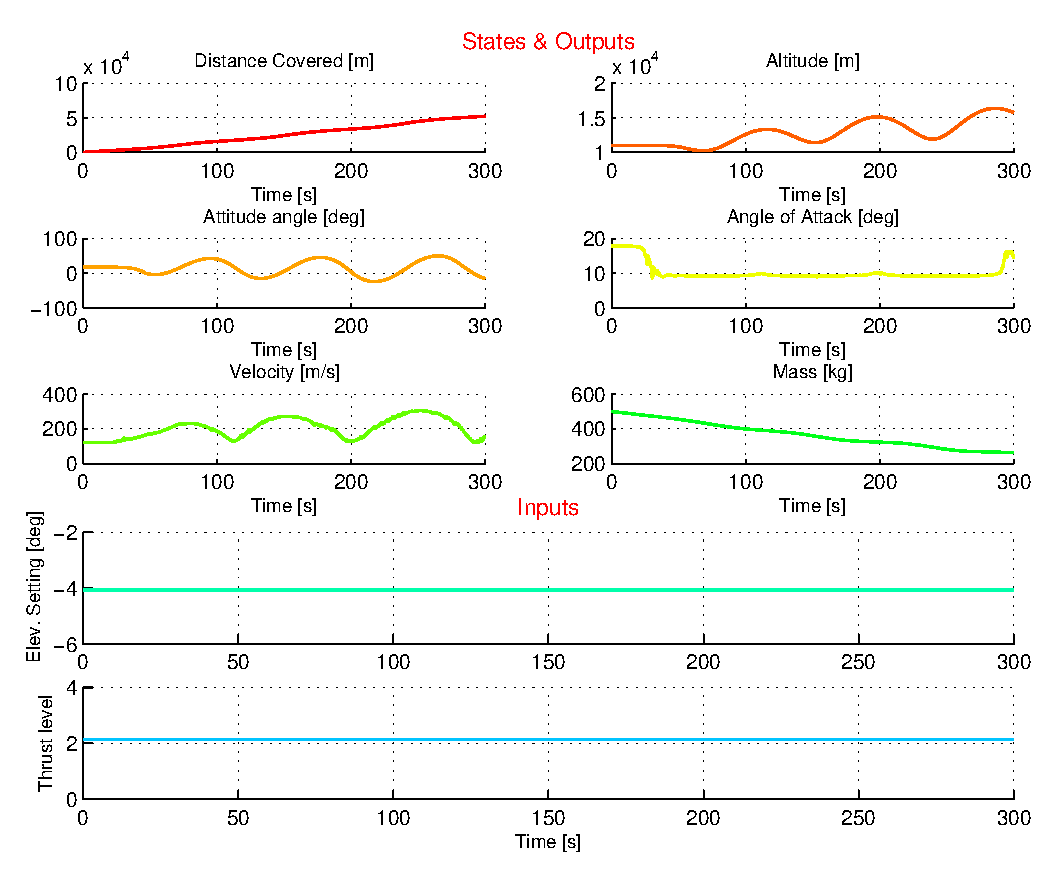
\includegraphics[width=1.0\textwidth]{nonlinear_sim}
    \caption{Simulation outcome for constant $\delta_e,\delta_p$}
    \label{fig:nonlinear_sim}
\end{figure}

As we can see, in the beginning (first 50s) aircrafts keeps a constant altitude
as wel as the other properties, but as the mass decreases, the aircraft starts
raising and velocity and attitude start oscilalting. The linear stability
analysis did not predict any divergence from the equilibrium point, because the
loss of mass was not included in the model.

An interesting point to make is that when the simulation is run with a
unacceptable cg position (e.g 10.3m) \textit{the altitude starts oscillating} with
increasing magnitude (see fig.\ref{fig:nonlinear2}) an indicator of unstable system behavior. If the xcg
increases even more, the time integration algorithm cannot find a valid solution
after a certain time.

\begin{figure}[H]
    \centering
    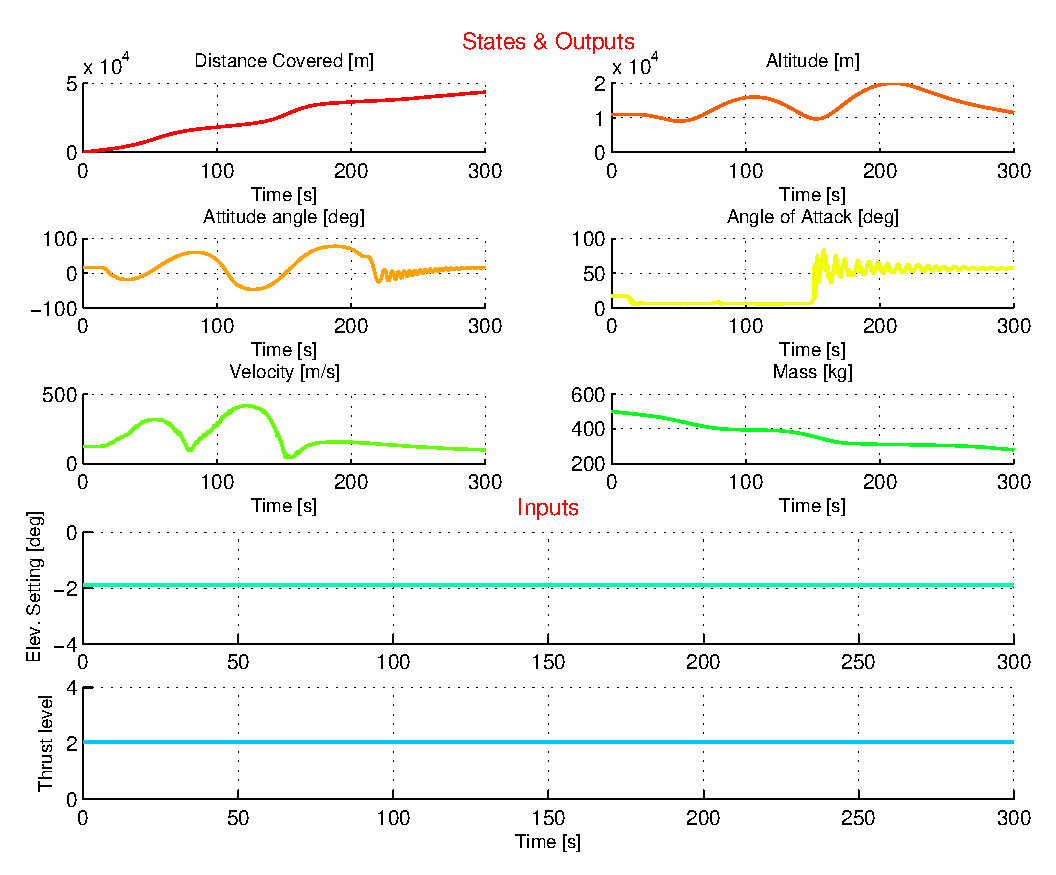
\includegraphics[width=1.0\textwidth]{nonlinear2}
    \caption{Nonlinear Simulation results for xcg = 10.3m}
    \label{fig:nonlinear2}
\end{figure}


\subsubsection{Looping}

The looping maneuver is perform by applying a negative elevator ($5-6\degree$) 
angle while having maximum thrust level. In this way the aircraft starts raising
in a curved trajectory until it reaches a maximum in an upside position. Then
maintaining the same elevator angle, after surpassing the max point of the
flight trajectory, we increase the thrust level so that when we reach the
initial altitude, we can maintain it in an equilibrium condition. 
\footnote{The elevator, thrust inputs are given in their respective csv files,
handed with the code}
The attempt of a loop maneuver is given 
in fig.~\ref{fig:looping}-\ref{fig:looping_status}


\begin{figure}[H]
    \centering
    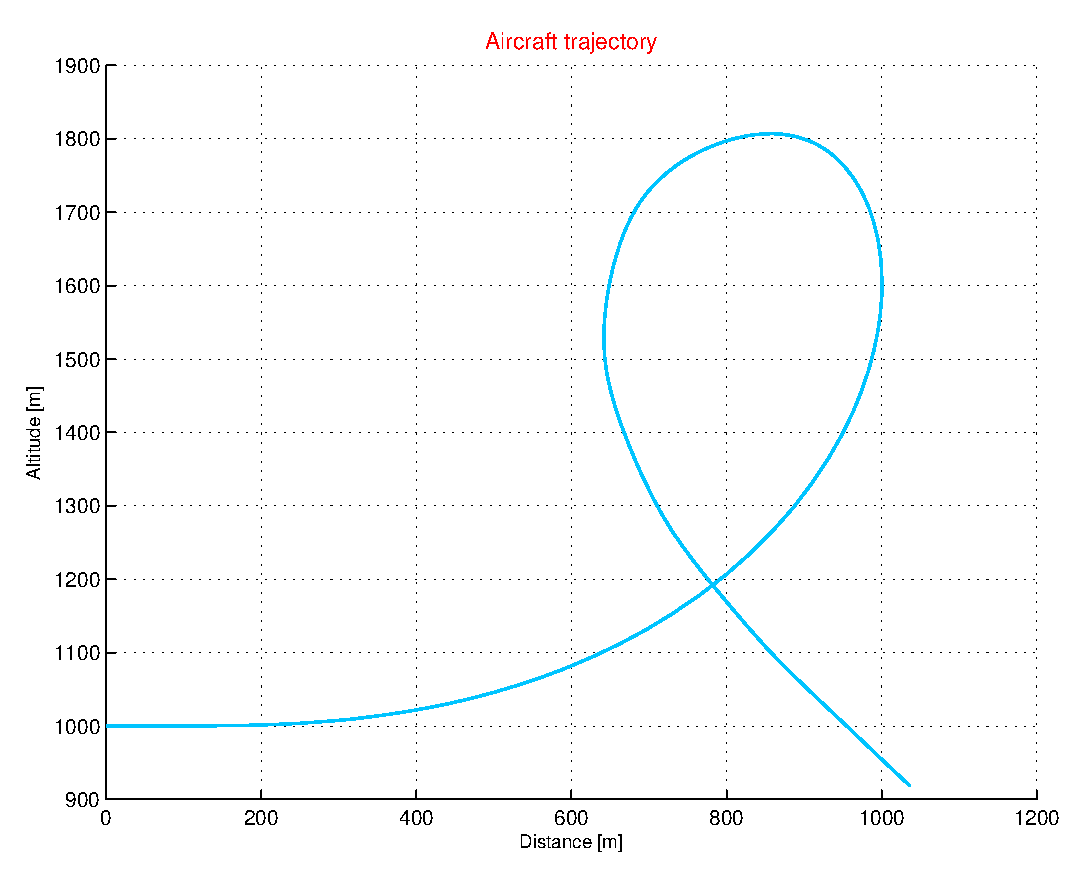
\includegraphics[width=\textwidth]{looping1}
        \caption{Looping Trajectory}
        \label{fig:looping}
\end{figure}
\begin{figure}[H]
    \centering
    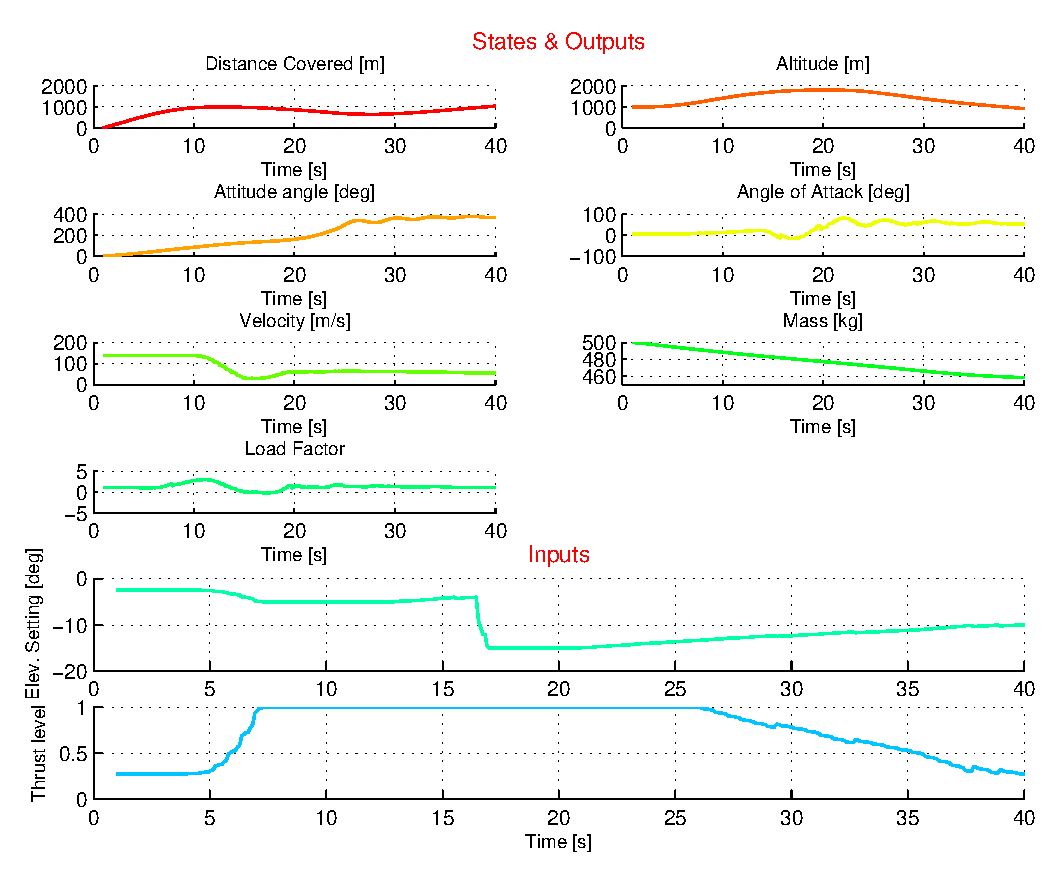
\includegraphics[width=\textwidth]{looping_status1}
    \caption{Parameters status during looping}
    \label{fig:looping_status}
\end{figure}

We can see that the roundness of the loop is sufficient, however we have
problems maintaining initial altitude after the loop.

\subsubsection{Cobra Maneuver}
In order to implement the cobra 

